\documentclass[../main.tex]{subfiles}
\graphicspath{{\subfix{../figures/}}}
\begin{document}
The theory part of the thesis is divided into four sections. Firstly, the model of the double dot system will be introduced in more detail. Then, a brief overview of the theory behind transport through quantum dots is given. The focus is then put on some of the tools used in open quantum systems, ultimately ending in a section about quantum master equations. The final section will further explain the notion of exceptional points, and introduce a couple of important tools used in exceptional point physics.
\subsection{The system}\label{sec:sys}
The system which was studied in this thesis is essentially given by figure~\ref{fig:model}, with a few assumptions and modifications. To reduce the dimension of the parameter space, a fixed tunneling rate $\Gamma$ and a variable tunneling detuning $\delta\Gamma$ are introduced. The four tunneling rates in terms of $\Gamma$ and $\delta\Gamma$ are assumed to be symmetrically given by figure~\ref{fig:model2}. It is also assumed that each dot is restricted to be either empty or contain one electron in the ground state of the dot. The energy of the ground state is given by a fixed gate voltage $V_\text{G}=0$ and a variable energy detuning $\delta\epsilon$: $\epsilon_{1/2} = -V_\text{G} \pm \delta\epsilon$. Furthermore, the temperatures of the leads $T_\text{L}=T_\text{R}=10\Gamma$, the chemical potentials $\mu_\text{L/R} = \pm V_\text{SD}/2$, the bias voltage $V_\text{SD} = 300\Gamma$, and the charging energy $U = 250\Gamma$, are all treated as constants. The charging energy being the extra energy needed to enter a quantum dot if the other dot is already occupied due to Coulomb interaction (?). This leaves the two tuning parameters, $\delta\Gamma$ and $\delta\epsilon$, as the only parameters of the system, resulting in a two dimensional parameter space. 

\begin{figure}[H]
    \centering
    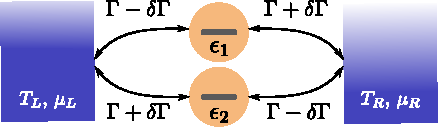
\includegraphics[width=0.8\linewidth]{figures/model.pdf}
    \caption{hej}
    \label{fig:model2}
\end{figure}

The full Hamiltonian of the system is given by $\hat H = \hat H_\text{QD} + \hat H_\text{leads} + \hat H_\text{coup}$ where the three terms correspond to the quantum dot, lead, and coupling Hamiltonians. By considering all the tunneling processes, these terms can be shown to be given by
\begin{equation}
    \begin{aligned}
        \hat H_\text{QD} &= (-V_\text{G} - \delta\epsilon) \hat d_1^\dag \hat d_1  +  (-V_\text{G} + \delta\epsilon)\hat d_2^\dag \hat d_2 + U\hat d_1^\dag \hat d_1 \hat d_2^\dag \hat d_2, \\
        \hat H_\text{leads} &= \sum_{k} (E_{L,k} \hat c_{L,k}^\dag \hat c_{L,k}  + E_{R,k} \hat c_{R,k}^\dag \hat c_{R,k}), \\
        \hat H_\text{coup} &= \sum_k (t_{L,1} \hat d_1^\dag \hat c_{L,k} + t_{L,2} \hat d_2^\dag \hat c_{L,k} + t_{R,1} \hat d_1^\dag \hat c_{R,k} + t_{R,2} \hat d_2^\dag \hat c_{R,k}) + \text{H.c},
    \end{aligned}
\end{equation}
where $\hat d_{1/2}^\dag$ creates an electron in dot 1 or 2, and $\hat c_{L/R,k}^\dag$ creates an electron in the left or right lead with quantum number $k$ and energy $E_{L/R,k}$. The tunneling amplitudes $t_{L/R,1/2}$ are directly related to the corresponding tunneling rates $\Gamma_{L/R,1/2}$. 

To be able to simulate the dynamics of the system, a couple more approximations have to be made regarding the coupling between the dots and the leads. (reasonable assumptions?) The first is to assume that the strength of the interaction between the system and the environment is weak. It is therefore possible to treat the interaction perturbatively in terms of the tunneling rate $\Gamma$. The second main approximation is to assume that the interaction between the system and the environment is Markovian. A Markovian process is one in which the next time step only depends on the current state of the system. In a quantum dot system, this can be interpreted to mean that the leads "forget" that they have lost or gained an electron, right after the tunneling process has happened. Since the number of electrons in the leads typically is large, this can be a reasonable approximation for such systems.

These last two assumptions are made to motivate the use of a common tool used to simulate open quantum systems, the Lindblad master equation. The next two sections will introduce the theory necessary to understand its uses and origin.

\subsection{Transport through quantum dots}
\subsubsection{A simple example}
To begin understanding the transport of electrons through a system of quantum dots, it is insightful to first study the single quantum dot system. The following explanation is inspired by reference~\cite{transport}.

Consider a single quantum dot with $N$ electrons capacitively coupled to a gate and coupled to source and drain reservoirs through tunnel junctions as in figure~\ref{fig:qdotscheme}. The main transport properties of the system can then be understood in terms of the chemical potentials of the quantum dot and the source and drain reservoirs. These are often depicted in electro-chemical potential diagrams, see figure~\ref{fig:ladder}. There, $\mu(N)$ is the energy required to add the $N$th electron to the quantum dot, and $\mu_S$ and $\mu_D$ are the Fermi levels of the source and drain. The shaded areas represent the Fermi-Dirac distributions of the source and drain.
\begin{figure}[H]
    \centering
    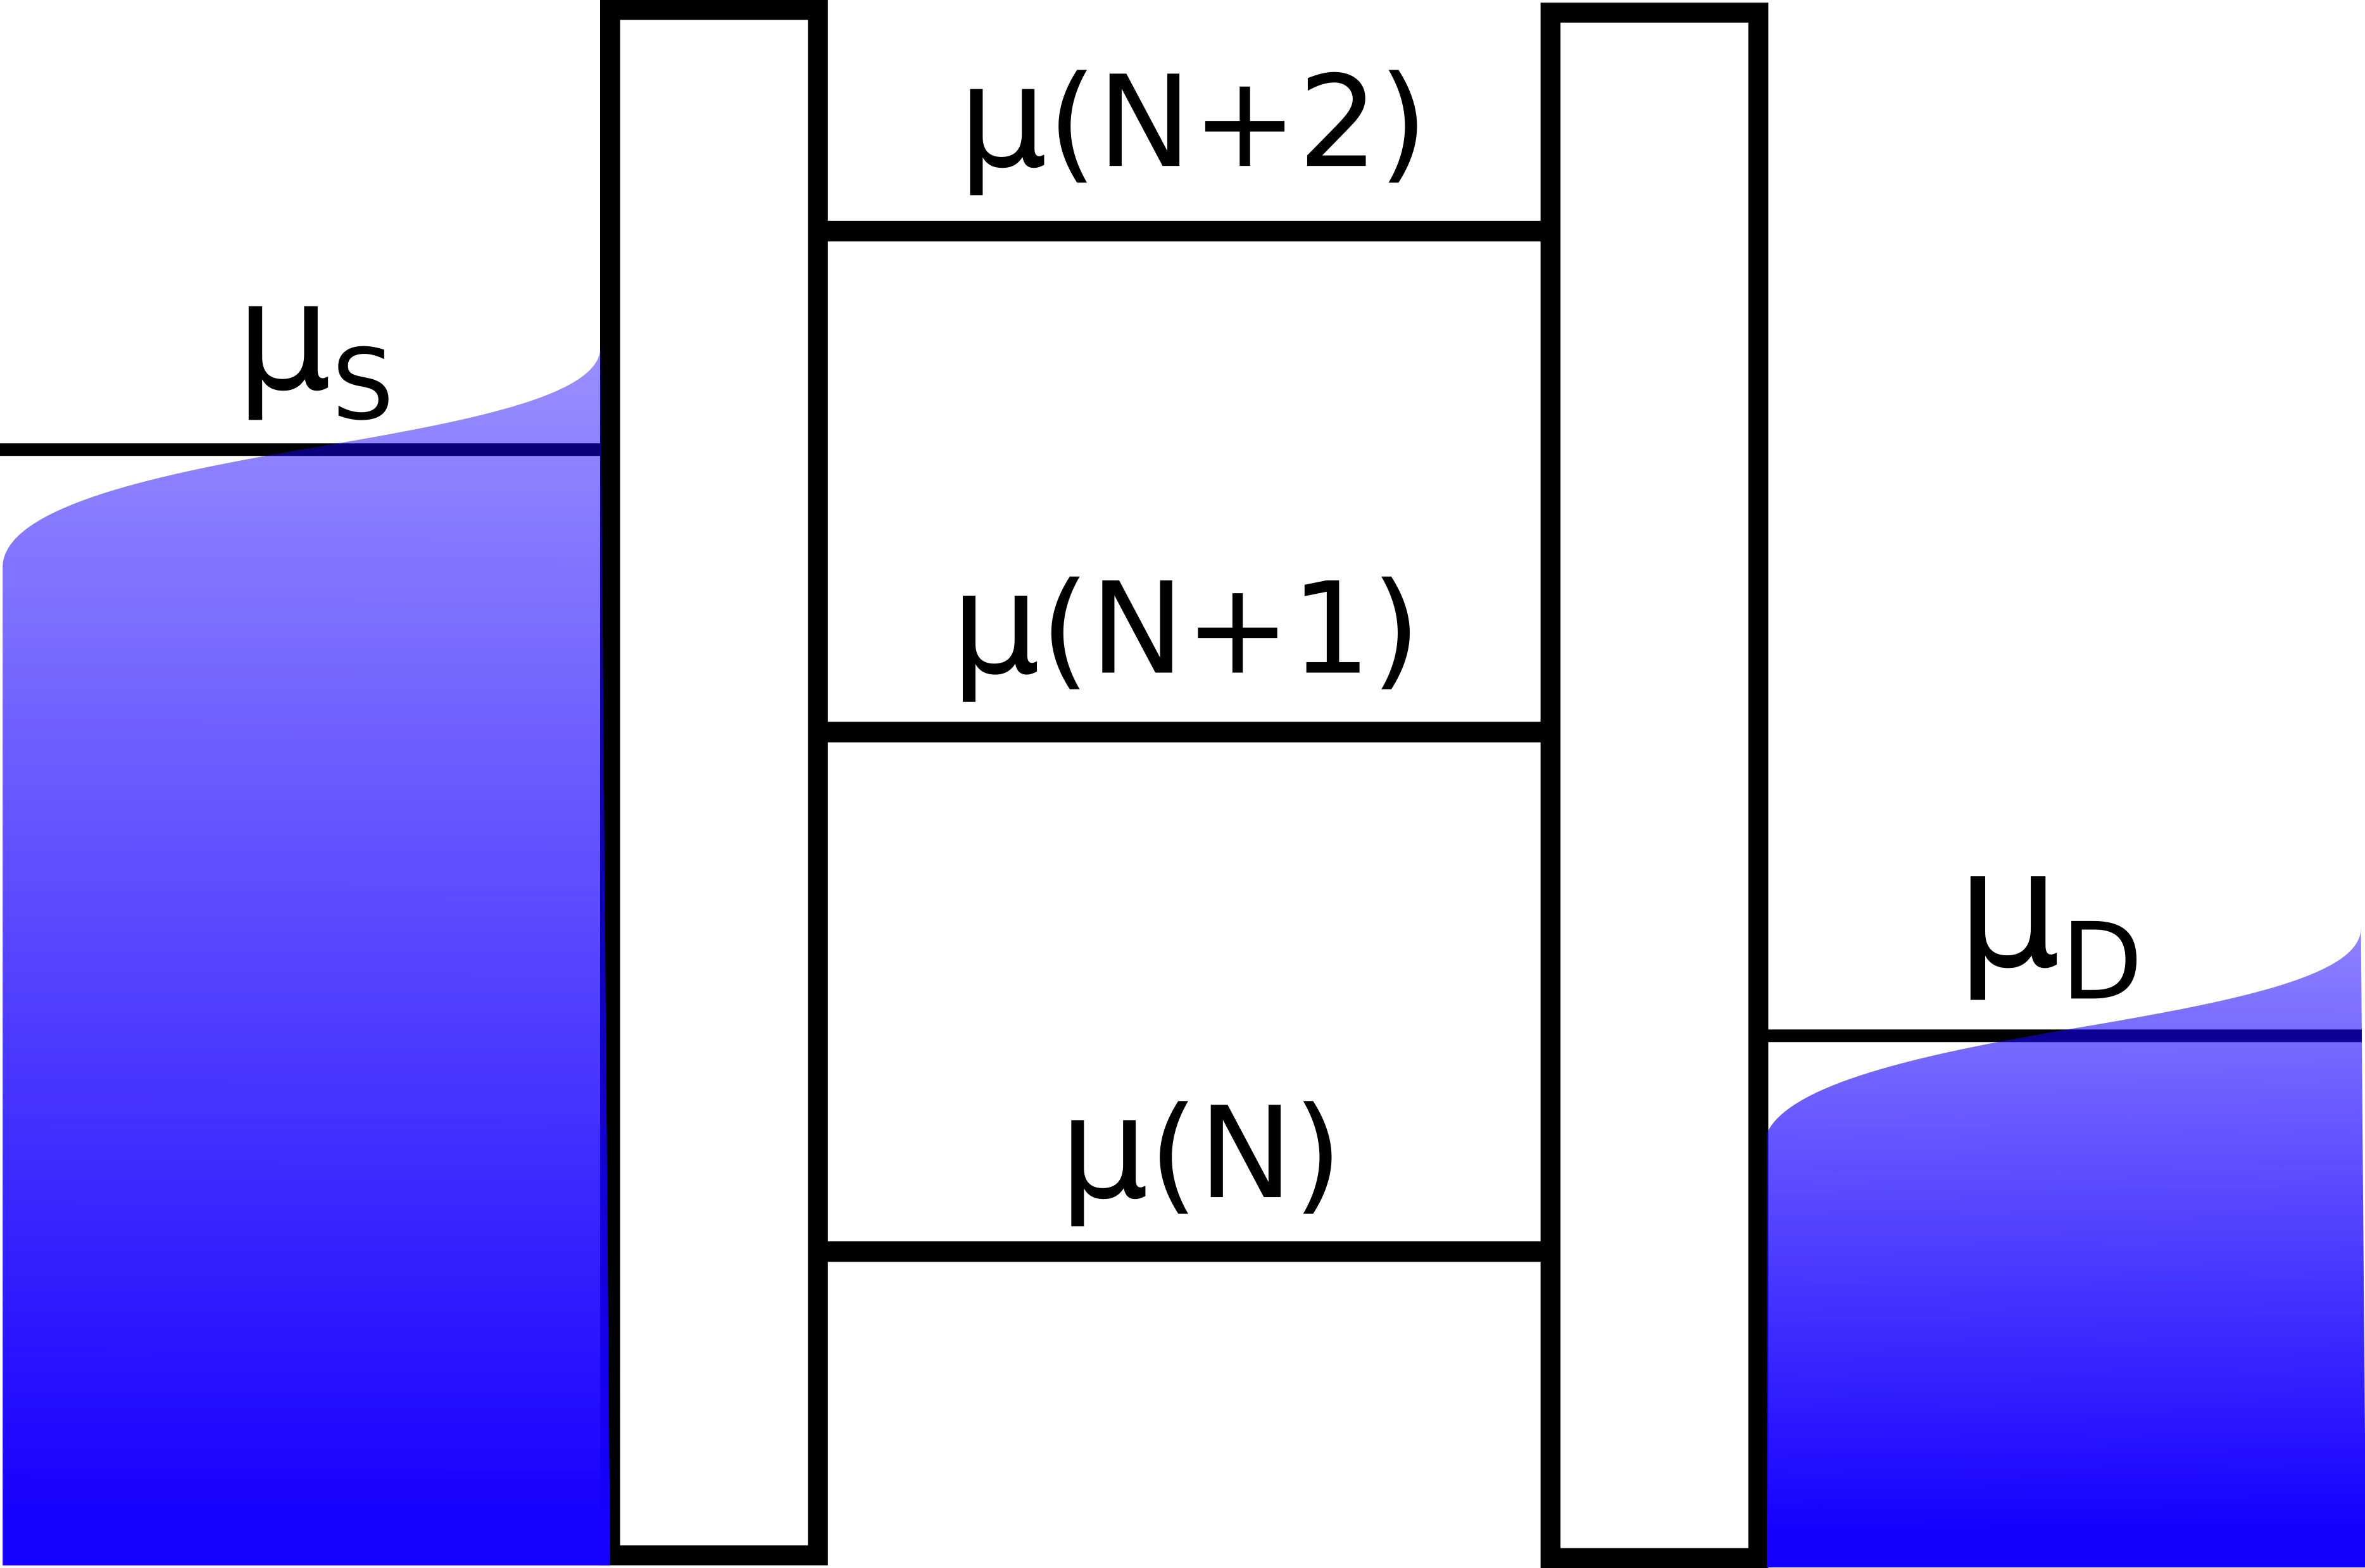
\includegraphics[width=0.6\linewidth]{figures/ladder.png}
    \caption{hej}
    \label{fig:ladder}
\end{figure}
Using this picture, the electron transport through the quantum dot can be easily visualized. If the chemical potential levels are located as in figure~\ref{fig:ladder}, $\mu(N + 1)$ is below $\mu_S$, and an electron will likely tunnel from the source onto the dot, increasing the number of electrons on the dot from $N$ to $N+1$. After the tunneling event, there is an even lower chemical potential available for the electron, $\mu_D$, and the electron will with a high probability leave the quantum dot and enter the drain. In this fashion, the system will cycle through having $N$ and $N+1$ electrons on the dot, producing a current.  

It turns out that $\mu(N)$ depends linearly on the gate voltage $V_G$, so by changing it, the "ladder" of states in figure~\ref{fig:ladder} can be lowered or raised. The drain voltage $V_D$ on the other hand, changes the spacing between $\mu_S$ and $\mu_D$. Through these two processes, it is possible to change the electro-chemical potential landscape and therefore control the current through the system. 

\subsubsection{Master equations}
An important tool for simulating the current through a quantum dot system is the master equation approach. A classical master equation is defined by
\begin{equation}\label{master}
    \diff{p_i}{t} = \text{Rate of entering state } i - \text{Rate of leaving state } i = \sum_j R_{ji}p_j  - \sum_j R_{ij}p_i
\end{equation}
with probabilities $p_i$ of being in state $i$, and transition rates $R_{ij}$ describing the rate of transitions from state $i$ to state $j$. For the single quantum dot system, the states $i$ correspond to the number of electrons on the dot. The transition rates are typically related to the Fermi-Dirac distributions of the reservoirs and the tunneling rates of the barriers~\cite{transport}.

Collecting the rate equations for each $i$ and adding the condition $\sum_i p_i = 1$, a system of ordinary differential equations is obtained. This can be solved numerically using standard methods, such as the Runge-Kutta method. Once the probabilities are obtained, the evolution of the current can be calculated by considering the amount of charge tunneling through the barriers at each time point~\cite{transport}.

While a classical master equation may give accurate results for some quantum systems, it leaves out some important physics. A quantum master equation generalizes the notion of a classical master equation in the following sense: The unknown in a quantum master equation does not only contain the probabilities $p_i$ of being in a quantum state $\ket{\psi_i}$, but also coherences, which are necessary to describe a quantum system fully. This topic will be developed in more detail in the following section.
\subsection{The theory of open quantum systems}
Open quantum systems are systems which are non-isolated and connected to some sort of environment. Often, it considers a total system consisting of the (sub)system of interest, and an environment. The total system is closed, and therefore it obeys the regular quantum mechanical equations of motion. The goal of the theory of open quantum systems is to infer the dynamics of the smaller system from the equations of the total system~\cite{lindblad}. 

\subsubsection{The von Neumann equation and the reduced density operator}

An important tool used in open quantum theory is the density operator $\hat{\rho}$. In open quantum systems, it might only be known that the system is in states $\ket{\psi_i}$ with probabilities $p_i$. Then the system is said to be in an ensemble $\{\ket{\psi_i}, p_i\}$. The density operator describes this information in a compact way:

\begin{equation}
    \hat{\rho} = \sum_i p_i \ket{\psi_i}\bra{\psi_i}.
\end{equation}

Fixing a basis $\{\ket{\phi_i}\}$, the density operator can be represented by a matrix with elements $\rho_{ij} = \braket{\phi_i|\hat\rho|\phi_j}$. The diagonal elements $\rho_{ii}$ represents classical probabilities of being in a state $\ket{\phi_i}$ and the off-diagonal elements $\rho_{ij}$ are the coherences of the system~\cite{bookopen}.
%The density operator is Hermitian, positive and has unit trace. 

The average measured value of an observable $\hat O$ of an ensemble represented by $\hat\rho$ can be shown to be given by equation~\eqref{exp}. From the density operator one can therefore extract all signifiant information from the ensemble, and it can be described as the "state" of the system.

\begin{equation}\label{exp}
    \braket{\hat O} = \tr({\hat\rho \hat O}).
\end{equation}

It is also possible to calculate how the density operator evolves over time. Under a Hamiltonian $\hat H$, the evolution is given by the von Neumann equation

\begin{equation}\label{vonneumann}
    i\hbar\diff{\hat\rho}{t} = [\hat H, \hat\rho] \equiv \mathcal{L}\hat\rho,
\end{equation}
where $\mathcal{L}$ is the Liouvillian superoperator, or just the Liouvillian~\cite{bookopen}. 

Returning to the mentioned goal of the theory of open quantum systems - How does one extract the density operator of a subsystem connected to an environment from the total density operator? This question is solved by the reduced density operator. If the total system $T$ consists of a subsystem $S$ and an environment $E$, then the reduced density matrix for the subsystem is given by

\begin{equation}
    \hat\rho_S = \tr_E({\hat\rho_T}),
\end{equation}
where $\tr_E$ is the partial trace over the environment. It is therefore possible to "trace out" the environment and obtain a density operator for the subsystem of interest. The reduced density operator contain all measurement statistics of interest in the subsystem, placing it at the core of the theory of open quantum systems~\cite{bookopen}.


\subsubsection{The Lindblad Master equation}\label{sec:lind}
The starting point for quantum master equations is the von Neumann equation (eq.~\eqref{vonneumann}) for the density matrix of the total system. Using the partial trace, a differential equation for the reduced density matrix $\hat\rho$ of the system of interest can be obtained. However, the resulting equation still includes the total density operator and is in most cases impossible to solve~\cite{lindblad}. The approximations required to find a solution can be done in many different ways and is essentially what differs the quantum master equations apart.

One of the most famous quantum master equations is the Lindblad equation. As described in section~\ref{sec:sys}, the Lindblad equation is based on two major approximations: that the system-bath interaction is Markovian, and weak. Applying these approximations to the von Neumann equation, the Lindblad equation can be derived:

\begin{equation}\label{eq:lind}
    \diff{\hat\rho}{t} = i[\hat\rho, \hat H_\text{eff}] + \sum_i \hat L_i\hat\rho\hat L_i^\dag - \frac{1}{2}\hat\rho\hat L_i^\dag\hat L_i - \frac{1}{2}\hat L_i^\dag\hat L_i \hat\rho \equiv \mathcal{L}\hat\rho,
\end{equation}
where $\hat H_\text{eff}$ consists of two terms: the subsystem Hamiltonian $\hat H_\text{S}$ and the Lamb shift Hamiltonian $\hat H_\text{LS}$, a renormalization of energy levels due to the interaction with the environment~\cite{lindblad}. The $\hat L_i$'s are the so called jump operators, which capture the coupling processes to the environment. ($\hbar=1$) One method for calculating the jump operators is described in reference~\cite{perlind}. There, a phenomenological approach is proposed. Using this so called PERLind approach, the jump operators are calculated using well defined steps, and can be applied in a wide range of systems. Once the jump operators are constructed and the first term of equation~\eqref{eq:lind} is calculated, an expression for the Liouvillian $\mathcal{L}$ can be obtained. Due to their dissipative nature, the last three terms of the Lindblad equation are non-unitary~\cite{bookopen}. The matrix representation of the full Liouvillian is therefore not necessarily Hermitian, which will enable the possibility of exceptional points.

\begin{enumerate}
    \item Explain that it preserves unity trace and positivity?
\end{enumerate}

%One of the attractive properties of the Lindblad equation is that it ensures the positivity and unity trace of the density operator throughout the evolution (explain in prev section). Other quantum master equations do not have this property, which may cause negative probabilities and other unphysical results.

\subsubsection{The Fock-Liouville space}
Where to put this?

The Liouvillian $\mathcal{L}$ in equation~\eqref{vonneumann} is an operator acting on an operator, which is why it is called a superoperator. To be able to more easily handle the Liouvillian, it is possible to treat it as a normal operator represented by a matrix, acting on a Hilbert space spanned by the density matrices. The density matrix is therefore effectively transformed into a vector, usually written as $\ket{\rho}\rangle$, with a scalar product $\langle\braket{\rho_1|\rho_2}\rangle$. The Hilbert space spanned by these vectors is called the Fock-Liouville space.


\subsection{Exceptional points}\label{sec:ep}
In quantum mechanics, a common way to simplify a calculation is to diagonalize the matrix representation of the operator describing the system. The diagonalization process can be understood a change of basis to linearly independent eigenvectors. In this basis, the linear transformation of the matrix is very simple: it scales each eigenvector by the corresponding eigenvalue. The matrix in the new basis is therefore diagonal, explaining the name of the process. For a matrix $A$ and its diagonal form $D$, this can be written as 
\begin{equation}
    A = SDS^{-1},
\end{equation}
where $S = (v_1, \dots ,v_n)$ consists of the eigenvectors of $A$~\cite{uffe}.

In Liouvillian physics, we have seen that there are non-unitary parts in the Liouvillian superoperator. The matrix representation of the Liouvillian is hence not necessarily diagonalizable, but can be defective. If a matrix is defective, two or more eigenvalues and their corresponding eigenvectors coalesce. If a point in the parameter space of the matrix corresponds to a defective matrix, the point is called an exceptional point~\cite{nonHermrev}. Exceptional points can be of different orders, reflecting how many eigenvectors coalesce at the point. The notion of exceptional points and its orders is related to a type of matrix decomposition, the Jordan normal form.

\subsubsection{Jordan normal form}

For a defective matrix, there does not exist a basis of eigenvectors, and the diagonalization process is not possible. Fortunately, there is a notion of an "almost diagonal" form, called the Jordan normal form. Recall that in the diagonalizable case, the basis was changed to the linearly independent eigenvectors. To construct the Jordan form for a defective matrix, this basis has to be completed in some way to span the full space. This can be done using Jordan chains, which for each defective eigenvector $r_i$ with eigenvalue $\lambda_i$, consists of vectors $r_i, r_i'$, $r_i'' \dots$ defined by equation~\eqref{jordanchain}~\cite{uffe}. The length of chain, $n_i$, is the same as the order of the corresponding EP.

\begin{equation}\label{jordanchain}
\begin{aligned}
    (A-\lambda_iI)r_i &= 0 \\
    (A-\lambda_iI)r_i' &= r_i \\
    (A-\lambda_iI)r_i'' &= r_i' \\
    &\vdots \quad.
\end{aligned}
\end{equation}
Using this new basis and creating the change-of-basis matrix $M$ by forming

\begin{equation}\label{chofba}
    M = (\boldsymbol{r}_1 \dots \boldsymbol{r}_q), \quad \text{where } \boldsymbol{r}_i = (r_i,\; r_i',\; r_i'' \dots), 
\end{equation}
the Jordan normal form $J$ of the matrix $A$ is obtained:

\begin{equation}
\begin{aligned}
    A &= MJM^{-1}, \\ \quad \text{where } J = \begin{bmatrix}J_{n_1}(\lambda_1) & \dots & 0 \\
                                                         \vdots & \ddots & \vdots \\
                                                         0 & \dots &  J_{n_q}(\lambda_q)\end{bmatrix} \quad
      &\text{and } J_{n_i}(\lambda_i) = \begin{bmatrix} \lambda_i & 1 & \dots & 0 \\
                                                                                        \vdots  & \ddots & \ddots & \vdots \\
                                                                                        \vdots & & \ddots& 1 \\
                                                                                        0 & \dots & \dots & \lambda_i\end{bmatrix}.
\end{aligned}
\end{equation}
The Jordan form hence consist of $q$ blocks on the diagonal, each block of size $n_i$ consisting of its eigenvalue on the diagonal and ones on the super diagonal~\cite{uffe}. Note that if all blocks are of size one, i.e there are no exceptional points, the Jordan form is diagonal.
\begin{enumerate}
    \item Perhaps mention the problems of calculating the Jordan form numerically?
    \item Explain how it can be done.
    \item Left eigenvectors in $M^{-1}$
\end{enumerate}

\subsubsection{Solution of ODEs for exceptional points}
An ordinary differential equation (ODE) is a linear differential equation of the form $x'=Ax$. Often, the unknown $x$ is a vector, and $A$ a matrix. The solution can be written as a matrix exponential in the following way:

\begin{equation}
    x(t) = e^{At}x(0), \;\text{where } \;e^{At} = \sum_{k=0}^{\infty}\frac{(At)^k}{k!}.
\end{equation}

The matrix exponential can be simplified using Jordan decomposition. It can be shown that  $e^{At} = Me^{Jt}M^{-1}$ where 

\begin{equation}
    \begin{aligned}
        e^{Jt} = &\begin{bmatrix}e^{J_{n_1}(\lambda_1)t} & \dots & 0 \\
                                                         \vdots & \ddots & \vdots \\
                                                         0 & \dots &  e^{J_{n_q}(\lambda_q)t}\end{bmatrix} \text{, and } \\
            e^{J_{n_i}(\lambda_i)t} = e^{\lambda_it} &\begin{bmatrix} 1 & t & \dots & t^{n_i-1}/(n_i-1)! \\
                                                                \vdots  & \ddots & \ddots & \vdots \\
                                                                \vdots & & \ddots& t \\
                                                            0 & \dots & \dots & 1\ \end{bmatrix}.
    \end{aligned}
\end{equation}

In general, the matrix exponential therefore consists of entries with terms of the form $t^ke^{\lambda_it}$~\cite{uffe}. Note that if $A$ is diagonalizable, all blocks are of size one and the entries consist of pure exponentials on the diagonal. 

Using this result, the solution can be written as 

\begin{equation}\label{jordanode}
    x(t) = Me^{Jt}M^{-1}x(0).
\end{equation}

This can further be decomposed if one considers the generalized modes of the system (FIND SOURCE). Suppose first that the initial state is in a linear combination of vectors in one of the Jordan chains, $x(0) = a_1r_i + a_2r_i' + a_3r_i'' + \dots = \boldsymbol{r}_ia$, where $a = (a_1, \dots a_{n_i})^T$ is a constant vector and $\boldsymbol{r}_i$ is defined in equation~\eqref{chofba}. By rewriting $M^{-1}$ as

\begin{equation}
    M^{-1} = \begin{bmatrix} \boldsymbol{l}_1 \\ \vdots \\ \boldsymbol{l}_{n_i} \end{bmatrix}
\end{equation}
and using equation~\eqref{jordanode}, the solution can be written as

\begin{equation}\label{genmode}
    x(t) = Me^{Jt}M^{-1}x(0) = Me^{Jt} \begin{bmatrix} \boldsymbol{l}_1 \\ \vdots \\ \boldsymbol{l}_{n_i} \end{bmatrix} \boldsymbol{r}_ia = \boldsymbol{r}_i e^{J_{n_i}(\lambda_i)t} a,
\end{equation}
since $\boldsymbol{l}_j\boldsymbol{r}_i = \delta_{ij}I$, where $I$ is the $n_j\times n_i$ identity matrix. Hence, the solution stays in the space spanned by the initial condition throughout the evolution. For an arbitrary initial condition, the solution can be written as a sum over the generalized modes: 

\begin{equation}
    x(t) = \sum_{i=1}^q \boldsymbol{r}_i e^{J_{n_i}(\lambda_i)t} \boldsymbol{l}_i x(0).
\end{equation}

\end{document}






